\documentclass[11pt,a4paper,openany]{report}
\usepackage[T1]{fontenc}
\usepackage[utf8]{inputenc}
\usepackage{lmodern}
\usepackage{microtype}
\usepackage{amsmath,amssymb,mathtools,bm}
\usepackage{booktabs,array,longtable,tabularx}
\usepackage{xcolor}
\usepackage[margin=23mm,headheight=23pt]{geometry}
\usepackage{enumitem}
\usepackage{fancyhdr}
\usepackage{fancyvrb}
\usepackage{graphicx}
\usepackage{url}
\usepackage{xurl}
\usepackage{hyperref}

\definecolor{finblue}{HTML}{1F5A99}
\definecolor{fingreen}{HTML}{19733A}
\definecolor{finorange}{HTML}{D55E00}
\definecolor{finred}{HTML}{A61B1B}
\definecolor{finviolet}{HTML}{6A3D9A}
\definecolor{fingray}{HTML}{4D4D4D}
\hypersetup{
  unicode=true,
  colorlinks=true,
  linkcolor=finblue,
  citecolor=fingreen,
  urlcolor=finblue,
  pdftitle={Atlas puzzli nadsolitona: audyt Z12 i dynamiczna redukcja},
  pdfauthor={Krzysztof Żuchowski},
  pdfsubject={Kontrolowana analiza międzydziedzinowa FIN, audyt symulatora Z12 i twierdzenie o pamięci generowanej przez dynamiczny Schur},
  pdfkeywords={FIN, Z12, spectral graph, Schur complement, memory kernel, Mori-Zwanzig, chirality, operator theory}
}
\pagestyle{fancy}
\fancyhf{}
\fancyhead[L]{\small Atlas puzzli nadsolitona}
\fancyhead[R]{\small Release 10.22}
\fancyfoot[C]{\thepage}
\setlength{\parindent}{0pt}
\setlength{\parskip}{0.55em}
\setlist{nosep,leftmargin=2em}
\setcounter{tocdepth}{2}
\setcounter{secnumdepth}{3}
\emergencystretch=3em

\newcommand{\one}{\bm 1}
\newcommand{\C}{\mathbb C}
\newcommand{\R}{\mathbb R}
\newcommand{\Z}{\mathbb Z}
\newcommand{\statusProven}{\textcolor{fingreen}{[Proven]}}
\newcommand{\statusStrong}{\textcolor{finblue}{[Strong evidence]}}
\newcommand{\statusModerate}{\textcolor{finviolet}{[Moderate evidence]}}
\newcommand{\statusWeak}{\textcolor{fingray}{[Weak evidence]}}
\newcommand{\statusSpeculative}{\textcolor{finorange}{[Speculative]}}
\newcommand{\statusRefuted}{\textcolor{finred}{[Refuted]}}

\begin{document}
\hypersetup{pageanchor=false}
\begin{titlepage}
\centering
\vspace*{12mm}
{\Large\bfseries FIN --- Release 10.22\par}
\vspace{12mm}
{\Huge\bfseries Atlas puzzli nadsolitona\par}
\vspace{6mm}
{\Large Audyt symulatora Z12, kontrolowana intuicja międzydziedzinowa\\
i nowy obiekt pamięci po redukcji\par}
\vspace{18mm}
{\Large Krzysztof \.Zuchowski\par}
\vspace{2mm}
{\normalsize Independent Researcher --- Fractal Information Theory Project\par}
\vspace{2mm}
{\normalsize ORCID: \href{https://orcid.org/0009-0002-0909-3613}{0009-0002-0909-3613}\par}
\vspace{10mm}
{\large 28 lipca 2026\par}
\vfill
\begin{minipage}{0.89\textwidth}
\small
\textbf{Główny wynik.} Dokładna eliminacja ukrytych węzłów strict \(Z_{12}\)
generuje zależną od częstotliwości samoenergię i proces z pamięcią.
Statyczne dopełnienie Schura jest tylko granicą resolwentową, a nie dokładnym
generatorem całej zredukowanej dynamiki.

\medskip
\textbf{Granica.} Wynik nie generuje selektora, jednostek fizycznych,
mostu legacy--strict ani walidacji eksperymentalnej.

\medskip
\textbf{Repozytorium.}
\url{https://github.com/hyconiek/Fractal-Nadsoliton-Theory}

\textbf{Licencja.} CC BY 4.0.
\end{minipage}
\vfill
\end{titlepage}
\hypersetup{pageanchor=true}
\pagenumbering{roman}
\tableofcontents
\clearpage
\pagenumbering{arabic}

\chapter*{Confidence convention}
\addcontentsline{toc}{chapter}{Confidence convention}

\begin{itemize}
\item 
\textbf{\statusProven{}} --- wynik algebraiczny albo numeryczny z jawnym testem i tolerancją.

\item 
\textbf{\statusStrong{}} --- stabilny w zadanej klasie testów, lecz nie jest twierdzeniem ogólnym.

\item 
\textbf{\statusModerate{}} --- sensowny mechanizm z niezamkniętą identyfikowalnością.

\item 
\textbf{\statusSpeculative{}} --- hipoteza badawcza, nie wniosek o naturze.

\item 
\textbf{\statusRefuted{}} --- teza sfalsyfikowana w zadanym modelu.

\end{itemize}

\chapter{Werdykt wykonawczy}

Najbardziej produktywne "uło\.zenie puzzli" nie prowadzi do nowego skalarnego parametru ani do ukrytego selektora. Prowadzi do obiektu operatorowego:

\[
\Sigma_E(z)=A_{EH}(zI+A_{HH})^{-1}A_{HE},
\]

czyli zale\.znej od częstotliwości \textbf{samoenergii zredukowanego procesu}, powstającej po rozdzieleniu węzłów na obserwowane \(E\) i ukryte \(H\). \statusProven{}

Ten obiekt łączy pięć wcześniej rozdzielonych obrazów:

\begin{enumerate}
\item 
Green/\allowbreak{}resolwent --- przez dokładną formułę blokowego resolwentu;

\item 
kompresję Schura --- jako granicę statyczną \(\Sigma_E(0)\);

\item 
dynamikę falową i dyfuzyjną --- przez tę samą analityczną rodzinę resolwentową;

\item 
pamięć i środowisko --- przez dokładne jądro pamięci w czasie;

\item 
obserwatora --- jako jawnie zadany podział dostępne/\allowbreak{}ukryte, a nie jako metafizyczny składnik równania.

\end{enumerate}

Nie rozwiązuje to jednak trzech głównych braków FIN: nie wybiera orientacji, nie generuje jednostki fizycznej i nie dostarcza eksperymentalnego przygotowania ani aparatu. \statusProven{}

Najgłębsza intuicja z atlasu brzmi więc:

\begin{quote}\itshape
Fraktalna redukcja nie powinna być modelowana wyłącznie jako statyczne przekształcenie jednego jądra w drugie. Dokładna eliminacja poziomu informacji generuje proces z pamięcią. Statyczny Schur jest tylko jego cieniem przy zerowej częstotliwości.

\end{quote}

Jest to dobrze znany mechanizm redukcji w matematyce fizycznej, ale jego konkretna postać dla ścisłego operatora FIN oraz połączenie z dualnością fala--dyfuzja stanowią nowy, testowalny kierunek wewnątrz projektu. Nie jest to dowód nowej fizyki.

\chapter{Metoda: intuicja z bezpiecznikami}

"Intuicyjne" porównanie mo\.ze łatwo zamienić podobieństwo obrazka w fałszywą równowa\.zność. Dlatego atlas został wykonany w czterech warstwach:

\begin{enumerate}
\item 
\textbf{Warstwa kształtu:} rozpoznanie podobnych wykresów, symetrii, przepływów i diagramów.

\item 
\textbf{Warstwa mechanizmu:} pytanie, czy obie struktury mają tę samą operację algebraiczną.

\item 
\textbf{Warstwa predykcji:} pytanie, czy analogia daje nową wielkość obliczalną i falsyfikowalną.

\item 
\textbf{Warstwa długu zało\.zeń:} wypisanie wszystkiego, co trzeba dodać, aby analogia stała się modelem fizycznym.

\end{enumerate}

Ka\.zde dopasowanie otrzymuje jeden ze statusów:

\begin{itemize}
\item 
\textbf{równowa\.zność ścisła} --- istnieje jawna mapa zachowująca działania;

\item 
\textbf{wspólny mechanizm} --- ta sama operacja, ale inne obiekty lub interpretacje;

\item 
\textbf{analogia strukturalna} --- podobna geometria albo widmo bez twierdzenia o równowa\.zności;

\item 
\textbf{metafora} --- pomocna wizualnie, bez mocy dowodowej;

\item 
\textbf{antyanalogia} --- podobieństwo ujawnia dokładnie miejsce, w którym FIN ró\.zni się od znanej teorii.

\end{itemize}

Skrypt fin\_nadsoliton\_puzzle\_atlas.py przeskanował:

\begin{itemize}
\item 
12 pojedynczych charakterystyk przeciw 15 dziedzinom: \textbf{180 porównań};

\item 
wszystkie nieuporządkowane pary charakterystyk: \(\binom{12}{2}=66\);

\item 
ka\.zdą parę przeciw 15 dziedzinom: \textbf{990 porównań}.

\end{itemize}

Łącznie wykonano \textbf{1170 jawnych indeksów podobieństwa}. Punktacja tagowa jest tylko narzędziem wyszukiwania kandydatów. Nie stanowi dowodu i nie jest u\.zywana do podnoszenia statusu hipotez.

\begin{figure}[htbp]
\centering
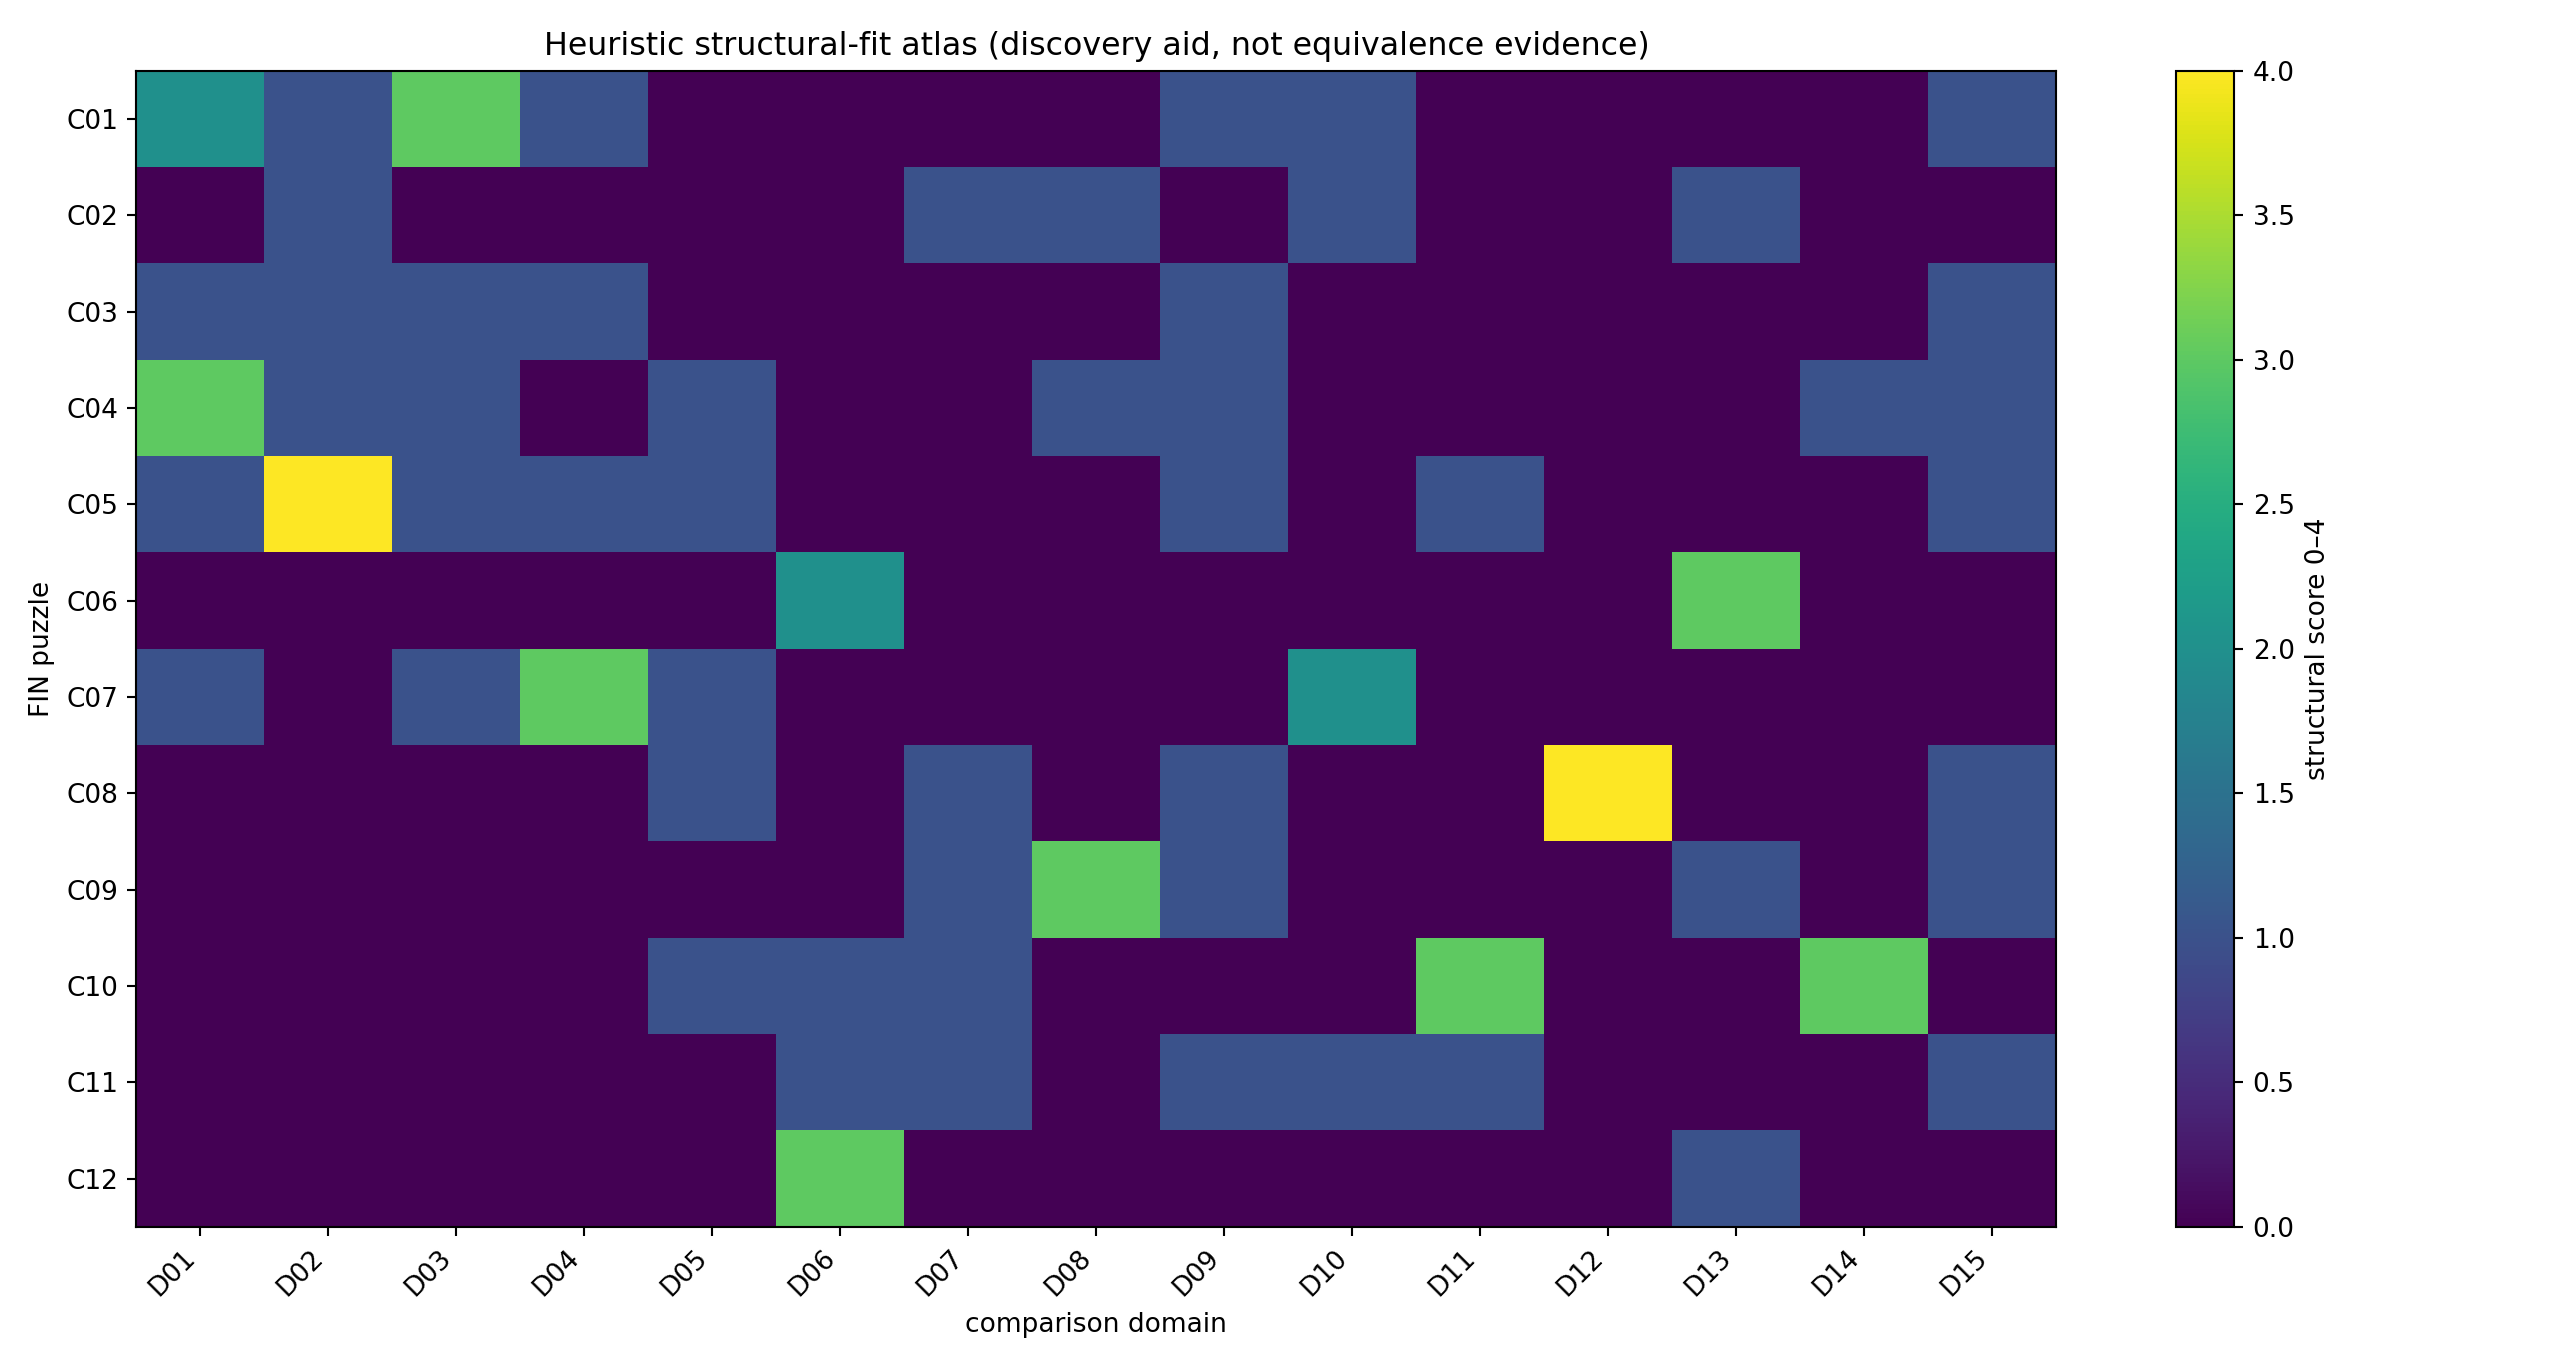
\includegraphics[width=0.96\textwidth]{FIN_Nadsoliton_Puzzle_Atlas_Figures/single_puzzle_domain_atlas.png}
\caption{Heurystyczna macierz dopasowania 12 puzzli do 15 dziedzin. Punktacja służy wyłącznie do wyszukiwania analogii.}
\end{figure}

\chapter{Co naprawdę robi kod Z12 sim.html}

Kod realizuje skończony eksperyment myślowy na \(Z_{12}\):

\[
W_{xy}=K(d(x,y)),\qquad
A=sI-W,\qquad
U_t=e^{-itA}.
\]

Stan początkowy jest częściowo koherentnym przygotowaniem dwóch węzłów:

\[
\rho_0(\phi,\eta)
=\frac12\Big(
|a\rangle\langle a|+|b\rangle\langle b|
+\eta e^{-i\phi}|a\rangle\langle b|
+\eta e^{i\phi}|b\rangle\langle a|
\Big).
\]

Po ewolucji \(\rho_t=U_t\rho_0U_t^\dagger\) kod oblicza:

\[
p_x(t)=(\rho_t)_{xx},
\qquad
J(x\to y)=2W_{xy}\operatorname{Im}(\rho_{yx}),
\]

oraz dwa ró\.zne sumaryczne obserwable prądu:

\[
C_1=\sum_xJ(x\to x+1),
\]

\[
C_\chi=\sum_x\sum_{d=1}^{5}d\,J(x\to x+d).
\]

\(C_1\) widzi wyłącznie pierwszą harmoniczną skoków. \(C_\chi\) jest zorientowanym prądem grupowym pełnego jądra z pominięciem krawędzi antypodalnej \(d=6\), której nie mo\.zna nadać znaku najkrótszego przesunięcia bez dodatkowej konwencji.

Zamysł kodu jest dobry: odró\.znić \textbf{odbiornik znaku} od \textbf{źródła znaku}. Radialny operator mo\.ze przenieść przygotowaną chiralność do mierzalnego prądu, ale nie wybiera sam znaku fazy.

\chapter{Błędy metodologiczne i wykonane poprawki}

\section{Niespójny znak prądu}

W dwóch składnikach diagonalnych kod obliczał przeciwny znak części urojonej ni\.z w składnikach interferencyjnych. To łamało jedną wspólną definicję \(J(x\to y)\).

\textbf{Poprawka:} wszystkie składniki są obecnie liczone jako

\[
2W_{xy}\operatorname{Im}(\rho_{yx}).
\]

\statusProven{}

\section{\texorpdfstring{Fałszywe twierdzenie o \(\eta=0\)}{Fałszywe twierdzenie o =0}}

Wygaszenie koherencji usuwa człony krzy\.zowe, lecz nie musi usuwać lokalnych prądów ka\.zdego z dwóch osobno propagowanych pakietów.

W teście:

\[
\max_{x,y}|J_{xy}|_{\eta=0}=0.0995050916,
\qquad
C_\chi|_{\eta=0}\approx0.
\]

\textbf{Poprawka:} interfejs mówi teraz, \.ze znika interferencyjna cyrkulacja, a nie wszystkie lokalne prądy. \statusProven{}

\section{Mylenie lokalnej harmonicznej z pełnym prądem}

Dla przygotowania \(a=10,b=2\):

\[
C_1(\phi)\approx0
\]

dla wszystkich badanych faz, chocia\.z pełny operator zawiera skoki dalekiego zasięgu. Dla \(\phi=0.7\):

\[
C_\chi=+0.1211880893,\qquad
C_\chi(-0.7)=-0.1211880893,
\]

podczas gdy

\[
C_1(0.7)=-2.36\times10^{-16}.
\]

\textbf{Poprawka:} symulator pokazuje \(C_\chi\) jako główny licznik i \(C_1\) jako kontrolę ślepej harmonicznej. \statusProven{}

\section{Niekanoniczna "cyrkulacja wszystkich krawędzi"}

Pierwotna suma wa\.zyła dalekie krawędzie przez arbitralnie zakodowane przesunięcie cykliczne, nie wyjaśniając wyboru gałęzi ani krawędzi antypodalnej.

\textbf{Poprawka:} obserwabla została zdefiniowana jawnie jako \(C_\chi\), wraz z informacją, \.ze zale\.zy od wybranej orientacji i podniesienia odległości. Jest detektorem chiralności, nie jej źródłem.

\section{Fałszywa "asymetria" przez zmianę rozstawu}

Para \(a=10,b=3\) nadal posiada odbicie zamieniające dwa jednakowe źródła. Przy \(\phi=0\) test daje \(C_\chi\approx0\).

\textbf{Poprawka:} przełącznik nazywa się "inna separacja", a nie łamanie symetrii. \statusProven{}

\section{\texorpdfstring{Fałszywa monotoniczność w \(|\phi|\)}{Fałszywa monotoniczność w ||}}

\(C_\chi\) jest funkcją nieparzystą i okresową:

\[
C_\chi(-\phi)=-C_\chi(\phi),\qquad
C_\chi(0)=C_\chi(\pi)=0.
\]

Mo\.ze rosnąć liniowo blisko zera, lecz nie globalnie w \(|\phi|\).

\textbf{Poprawka:} narracja i wykres opisują zachowanie okresowe. \statusProven{}

\section{Rozjazd widma i jądra}

Widmo \(A\) było wklejoną tablicą, więc zmiana \(K\) mogła pozostawić stare wartości własne.

\textbf{Poprawka:} widmo jest obecnie obliczane z jądra metodą Fouriera, a strona testuje:

\[
s=1.660307278766099,\qquad
\lambda_{\min}(A)\approx0,\qquad A\succeq0.
\]

\section{Brak kontroli równania ciągłości}

\textbf{Poprawka:} strona kontroluje normalizację i

\[
\dot p_x+\sum_yJ(x\to y)=0.
\]

Niezale\.zny audyt NumPy daje maksymalny residual \(5.55\times10^{-17}\).

\section{Mylące elementy wizualne}

Środkowa strzałka obracała się nawet dla zerowego prądu, a skala licznika zale\.zała od historii interakcji.

\textbf{Poprawka:} zero jest statyczne, a skala pochodzi deterministycznie z bie\.zącej krzywej \(C_\chi(\phi)\).

\section{Werdykt audytu}

audit\_z12\_sim.py przechodzi \textbf{15/\allowbreak{}15 testów}. \statusProven{}

Nie oznacza to, \.ze symulator dowodzi fizyczności FIN. Dowodzi tylko spójności zadeklarowanego skończonego modelu.

\chapter{Dwanaście pojedynczych puzzli}

\begin{center}
\begingroup\footnotesize
\setlength{\tabcolsep}{3.5pt}
\renewcommand{\arraystretch}{1.16}
\begin{longtable}{@{}p{0.055\textwidth}p{0.293\textwidth}p{0.187\textwidth}p{0.163\textwidth}p{0.163\textwidth}@{}}
\toprule
\textbf{ID} & \textbf{Charakterystyka FIN} & \textbf{Najbli\.zsze znane schematy} & \textbf{Co jest wspólne} & \textbf{Najwa\.zniejsza ró\.znica} \\
\midrule
\endhead
C01 & ścisłe jądro oscylacyjno-tłumione & spectral graph theory, graph signal processing, band-pass kernels & radialny filtr i widmo Fouriera & brak samodzielnego kontinuum i interpretacji fizycznej \\
C02 & legacy jako pośredni profil mostu & ekranowane funkcje Greena, propagatory oscylacyjne & oscylacja, tłumienie, amplituda & nie wolno przenosić ról legacy na strict bez twierdzenia \\
C03 & dodatni Laplasjan \(A\) & sieci przewodzące, procesy Markowa, Dirichlet forms & dodatniość, zachowanie stałej, energia gradientowa & czas i jednostki są bezwymiarowe \\
C04 & dualność \(e^{-itA}\) i \(e^{-tA}\) & quantum walks, heat kernels, Wick-like analytic continuation & wspólny rachunek funkcyjny & wspólny generator nie czyni procesów operacyjnie identycznymi \\
C05 & Green, resolwent i działanie & Gaussian fields, inverse field theory, Yukawa-type propagation & odwrotność operatora i działanie kwadratowe & interakcje, miara i skala działania są dodatkowymi danymi \\
C06 & cocykl orientacji i chiralne odbiorniki & cohomology, holonomy, topological phases, asymmetry resources & nośnik znaku i transformacja pod odbiciem & istnieją pary \(\pm\), lecz brak wybranego znaku \\
C07 & fraktalna kompresja Schura & Kron reduction, multigrid, RG, tensor networks & eliminacja stopni swobody & rodzina strict nie jest zamknięta pod audytowanym Schurem \\
C08 & adaptacyjny operator i pamięć & neural operators, reservoir computing, adaptive control & sprzę\.zenie zwrotne i stan pamięci & prawo uczenia i cel nie są wyprowadzone z strict \\
C09 & informacja i geometria & diffusion maps, Fisher geometry, optimal transport & metryki z rozkładów i semigrup & metryka wewnętrzna nie jest metrem SI \\
C10 & stan--zegar--instrument--rekord & process tensors, causal models, system identification & interwencje i wieloczasowe rekordy & konkretna aparatura pozostaje zewnętrzna \\
C11 & brak skali wymiarowej & dimensional analysis, renormalization, calibration theory & orbita skalowa i potrzeba standardu & bez kotwicy wymiarowej nie ma masy, energii ani czasu SI \\
C12 & brak selektora & spontaneous symmetry breaking, reference frames, resource theory & wielość gałęzi i koszt asymetrii & bifurkacja daje wiele gałęzi, nie kanoniczny wybór jednej \\
\bottomrule
\end{longtable}
\endgroup
\end{center}

\chapter{Układy kilku puzzli}

\section{Rdzeń widmowy: C01 + C03 + C04}

To układ najbli\.zszy skończonej teorii transportu na grafie. \statusProven{}

\begin{itemize}
\item 
\(W\) definiuje geometrię połączeń.

\item 
\(A=sI-W\) definiuje energię Dirichleta.

\item 
\(e^{-itA}\) daje propagację koherentną.

\item 
\(e^{-tA}\) daje relaksację/\allowbreak{}dyfuzję.

\end{itemize}

Równowa\.zność jest ścisła na poziomie rachunku funkcyjnego, ale nie na poziomie eksperymentalnych rekordów.

\section{Propagator odwrócony w działanie: C01 + C03 + C05}

Jeśli \(G=(L+m^2I)^{-1}\), to minimalne działanie kwadratowe

\[
S[\phi]=\frac12\phi^\top(L+m^2I)\phi-J^\top\phi
\]

ma równanie stacjonarne \((L+m^2I)\phi=J\) i odpowiedź \(\phi=GJ\). \statusProven{}

To jest poprawna rekonstrukcja działania z propagatora. Nie jest unikalnym prawem fundamentalnym, poniewa\.z mo\.zna dodać interakcje, miary i sektory niewidoczne w dwupunktowym Greenie.

\section{Chiralność jako zasób: C06 + C12}

Najbli\.zszą dziedziną jest teoria zasobów asymetrii. Operacje kowariantne względem odbicia nie tworzą asymetrii ze stanu odbiciowo symetrycznego. Przygotowana faza \(\phi\) jest zasobem; \(C_\chi\) jest odbiornikiem. \statusProven{}

To wyjaśnia, dlaczego symulator mo\.ze odczytać znak, lecz nie mo\.ze rozładować QW-2191.

\section{Informacja jako geometria: C04 + C09}

Semigrupa cieplna definiuje odległości dyfuzyjne i wieloskalowe współrzędne spektralne. To bliskie diffusion maps. \statusStrong{}

Antyanalogia jest kluczowa: z \(P_t\) mo\.zna otrzymać geometrię \textbf{bezwymiarową}, lecz nie metr, sekundę ani energię bez kalibracji.

\section{Operacyjny obserwator: C04 + C10}

Ten sam \(A\) nie wystarcza do określenia obserwowanego procesu. Potrzebne są:

\[
(\mathcal H,\rho,\mathcal E_t,\tau,\mathcal P,\mathcal I,\mathcal E,
\mathcal A,\mathcal R,\mathcal C,\mathcal D).
\]

Stan, interwencja, środowisko i zapis rozstrzygają, czy rekord wygląda falowo, dyfuzyjnie czy jak proces z pamięcią. \statusProven{}

\section{Statyczna kompresja: C05 + C07}

Schur/\allowbreak{}Kron daje dokładną odpowiedź brzegową przy ustalonym parametrze resolwentu. Jest to równowa\.zność blokowej algebry, nie dowód samopodobieństwa strict. \statusProven{}

Audytowane wcześniej niezamknięcie rodziny strict pod Schurem pozostaje w mocy.

\section{Dynamiczna kompresja: C04 + C05 + C07 + C10}

To najbogatsze nowe zestawienie. Gdy część węzłów jest niewidoczna, dokładny proces obserwowany nie jest generowany przez jeden statyczny Schur. Zamiast niego pojawia się \(\Sigma_E(z)\) i pamięć. \statusProven{}

\section{Fraktalność plus pamięć: C07 + C08}

Je\.zeli kolejne warstwy są eliminowane, ka\.zda warstwa wnosi własną samoenergię i jądro pamięci. Powstaje hierarchia:

\[
\Sigma^{(1)}(z),\Sigma^{(2)}(z),\ldots
\]

Mo\.ze ona przypominać continued fractions, multiscale impedance albo hierarchiczne modele pamięci. \statusModerate{}

Nie udowodniono, \.ze hierarchia odtwarza strict kernel ani wykładnik \(9/5\).

\section{Adaptacja plus proces z pamięcią: C08 + C10}

Adaptacyjny operator uczący się z rekordów procesu jest bliski identyfikacji układów z pamięcią i neural operators. \statusModerate{}

Ryzyko: model mo\.ze dopasować aparat zamiast FIN. Konieczne są kontrole permutacyjne, hold-out i identyfikowalność.

\section{Dwie niezale\.zne przeszkody: C11 + C12}

Brak skali i brak orientacji są ró\.znymi torsorami:

\begin{itemize}
\item 
skala: działanie \(\mathbb R_{>0}\);

\item 
orientacja: działanie \(\mathbb Z_2\) albo odpowiedniej grupy automorfizmów.

\end{itemize}

Skalar dodatni nie wybierze znaku, a pseudoskalar nie wygeneruje jednostki długości. \statusProven{}

To wyklucza częsty skrót myślowy, w którym jedna "stała informacyjna" miałaby jednocześnie tworzyć jednostki i selektor.

\section{Legacy + Green + strict: C02 + C05 + C01}

Legacy mo\.ze być oglądane jako pośredni profil propagatorowy, a strict jako późniejsze wzbogacenie. \statusModerate{}

Nie istnieje jednak licencja na:

\begin{itemize}
\item 
ciche zastąpienie legacy przez strict;

\item 
przeniesienie ról fizycznych legacy;

\item 
uznanie amplitudy albo tłumienia za pełną mapę ukończenia.

\end{itemize}

\section{Widmowe działanie: C03 + C05 + C09}

Ślad \(f(A/\Lambda)\) przypomina zasadę działania spektralnego, ale sama macierz \(A\) nie jest pełnym tripletem spektralnym i FIN nie generuje \(\Lambda\). \statusModerate{}

To cenna antyanalogia: znana teoria pokazuje dokładnie, jakie dodatkowe obiekty są potrzebne --- algebra, reprezentacja, operator typu Diraca, grading/\allowbreak{}real structure oraz skala.

\chapter{Nowe twierdzenie robocze: dynamiczny Schur generuje pamięć}

Podzielmy przestrzeń na węzły obserwowane \(E\) i ukryte \(H\):

\[
A=
\begin{pmatrix}
A_{EE}&A_{EH}\\
A_{HE}&A_{HH}
\end{pmatrix}.
\]

\section{Twierdzenie 1 --- dokładny blok resolwentu}

Dla \(z>0\):

\[
\left[(zI+A)^{-1}\right]_{EE}
=
\left[
zI+A_{EE}
-A_{EH}(zI+A_{HH})^{-1}A_{HE}
\right]^{-1}.
\]

Zatem:

\[
\Sigma_E(z)=A_{EH}(zI+A_{HH})^{-1}A_{HE}.
\]

\textbf{Dowód.} Jest to formuła odwrotności macierzy blokowej przez dopełnienie Schura. \statusProven{}

\section{Twierdzenie 2 --- brak jednego dokładnego statycznego generatora redukcji}

Dla \(z>0\):

\[
\Sigma_E'(z)
=
-A_{EH}(zI+A_{HH})^{-2}A_{HE}\preceq0.
\]

Jeśli sprzę\.zenie z ukrytym sektorem jest niezerowe w aktywnym kierunku, \(\Sigma_E'(z)\neq0\). Wtedy nie istnieje stała macierz \(B\), dla której

\[
\left[(zI+A)^{-1}\right]_{EE}=(zI+B)^{-1}
\]

dla wszystkich \(z>0\).

\textbf{Dowód.} Prawa strona wymagałaby

\[
B=A_{EE}-\Sigma_E(z)
\]

niezale\.znego od \(z\), co przeczy \(\Sigma_E'(z)\neq0\). \statusProven{}

\section{Twierdzenie 3 --- dokładny defekt składania po projekcji}

Niech \(P\) wybiera sektor \(E\), \(Q=I-P^\ast P\), a \(T(t)\) będzie albo \(e^{-tA}\), albo \(e^{-itA}\). Wtedy:

\[
PT(t+s)P^\ast
-PT(t)P^\ast PT(s)P^\ast
=
PT(t)QT(s)P^\ast.
\]

Prawa strona jest amplitudą albo masą trajektorii, które opuściły sektor obserwowany i wróciły. \statusProven{}

\section{Postać czasowa}

Dla dynamiki cieplnej:

\[
\dot x=-A_{EE}x-A_{EH}h,\qquad
\dot h=-A_{HE}x-A_{HH}h.
\]

Po dokładnym wyeliminowaniu \(h\):

\[
\dot x(t)
=-A_{EE}x(t)
+\int_0^t
M_E(t-s)x(s)\,ds
-A_{EH}e^{-tA_{HH}}h(0),
\]

\[
M_E(t)=A_{EH}e^{-tA_{HH}}A_{HE}.
\]

To jest równanie z pamięcią. "Środowisko" nie zostało dopisane --- powstało matematycznie z zadeklarowanego podziału na widoczne i ukryte stopnie swobody. \statusProven{}

\section{\texorpdfstring{Wynik dla strict \(Z_{12}\)}{Wynik dla strict Z\_12}}

Wybrano:

\[
E=\{0,2,4,6,8,10\},\qquad
H=\{1,3,5,7,9,11\}.
\]

\begin{center}
\begingroup\small
\setlength{\tabcolsep}{3.5pt}
\renewcommand{\arraystretch}{1.16}
\begin{longtable}{@{}p{0.420\textwidth}p{0.420\textwidth}@{}}
\toprule
\textbf{Test} & \textbf{Wynik} \\
\midrule
\endhead
residual sum wierszy statycznego Schura & \(2.78\times10^{-16}\) \\
maksymalny residual to\.zsamości resolwentowej & \(3.83\times10^{-15}\) \\
\(\|\Sigma'(0.05)\|_2\) & \(0.919783\) \\
\(\|\Sigma'(1)\|_2\) & \(0.290955\) \\
defekt składania heat przy \(t=0.5\) & \(0.119015\) \\
defekt składania wave przy \(t=0.5\) & \(0.305427\) \\
błąd statycznego Schura dla heat przy \(t=1\) & \(0.451941\) \\
błąd statycznego Schura dla wave przy \(t=1\) & \(0.921176\) \\
residual dokładnej to\.zsamości ukrytych wycieczek & \(<6.3\times10^{-16}\) \\
\bottomrule
\end{longtable}
\endgroup
\end{center}

\begin{figure}[htbp]
\centering
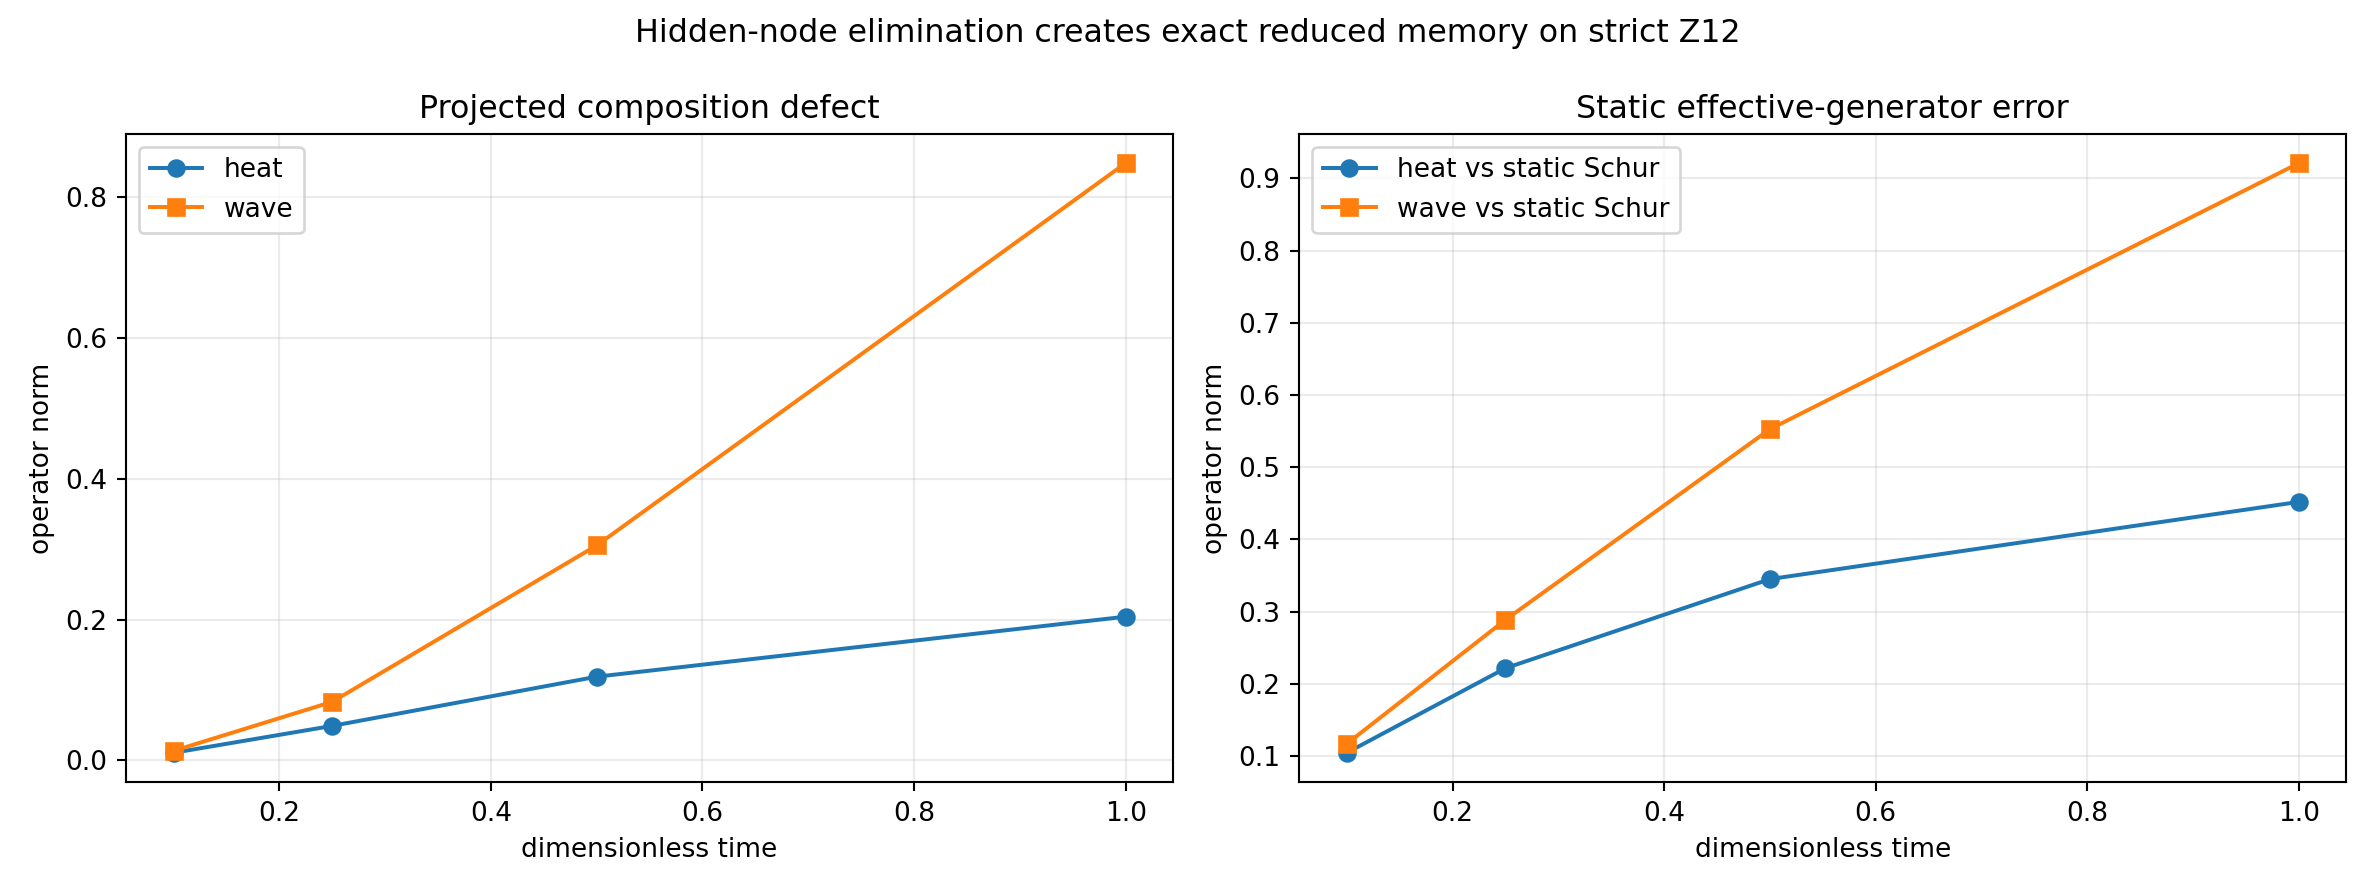
\includegraphics[width=0.96\textwidth]{FIN_Nadsoliton_Puzzle_Atlas_Figures/dynamic_schur_memory.png}
\caption{Defekt składania zredukowanych propagatorów i błąd zastąpienia dynamicznej redukcji jednym statycznym generatorem Schura.}
\end{figure}

\section{Znaczenie}

\begin{itemize}
\item 
\statusProven{} Fraktalna eliminacja stopni swobody generuje pamięć nawet wtedy, gdy pełna dynamika jest jednorodną semigrupą albo grupą.

\item 
\statusProven{} Fala i dyfuzja dzielą ten sam blokowy obiekt resolwentowy, lecz mają ró\.zne rekordy czasowe.

\item 
\statusModerate{} \(\Sigma_E(z)\) jest dobrym kandydatem na brakujący matematyczny interfejs między kompresją, środowiskiem i aparatem.

\item 
\statusRefuted{} Statyczne \(A_{\mathrm{Schur}}\) nie jest dokładnym generatorem całej zredukowanej dynamiki dla testowanego podziału.

\item 
\statusRefuted{} Pamięć po redukcji nie dowodzi fundamentalnego kierunku czasu ani świadomego obserwatora.

\end{itemize}

\chapter{"Kształty cieni" --- nowe intuicje}

\section{Brakujący obiekt mo\.ze być defektem przemienności}

Wiele niezamkniętych elementów ma wspólną postać:

\[
\text{najpierw redukuj, potem ewoluuj}
\neq
\text{najpierw ewoluuj, potem redukuj}.
\]

Defekt tej przemienności jest obserwowalnym cieniem ukrytych stopni swobody. \statusStrong{}

\section{Obserwator jest sekcją procesu, nie dodatkową substancją}

Matematycznie obserwator mo\.ze oznaczać:

\begin{itemize}
\item 
wybór podalgebry dostępnych obserwabli;

\item 
wybór projekcji \(P\);

\item 
zbiór dozwolonych instrumentów;

\item 
sposób zapisu wieloczasowego rekordu.

\end{itemize}

To nie dodaje "warstwy informacji pod nadsolitonem". Jest operacyjnym przekrojem stanów nadsolitona. \statusModerate{}

\section{\texorpdfstring{\(C_\chi\) i chiralny bispectrum są odbiornikami tego samego typu zasobu}{C\_ i chiralny bispectrum są odbiornikami tego samego typu zasobu}}

Oba są nieparzyste pod inwersją i zmieniają znak wraz z przygotowaniem. Mogą nale\.zeć do wspólnej klasy monotonicznych odbiorników asymetrii. \statusModerate{}

Nie wynika z tego, \.ze którykolwiek z nich wybiera znak.

\section{Ró\.zne obserwable widzą ró\.zne harmoniczne}

Ślepotę \(C_1\) przy niezerowym \(C_\chi\) nale\.zy potraktować jako ogólną lekcję tomograficzną. Pojedynczy prąd albo pojedynczy obraz interferencyjny nie identyfikuje pełnego operatora. \statusProven{}

\section{Statyczna samopodobność i dynamiczna samopodobność to ró\.zne hipotezy}

Brak zamknięcia strict pod statycznym Schurem nie wyklucza prostszej struktury dla rodziny \(\Sigma^{(n)}(z)\). To nowa, dobrze typowana hipoteza. \statusSpeculative{}

\section{Skala mo\.ze być względna, ale eksperyment wymaga kotwicy}

Stosunki widmowe są identyfikowalne bez absolutnego zegara. Absolutne energie i czasy nie są. \statusProven{}

Dlatego najpierw mo\.zna testować projective fingerprint, lecz fizyczna teoria nadal potrzebuje kalibracji.

\section{Informacyjna geometria mo\.ze być prawdziwa bez bycia czasoprzestrzenią}

Heat kernel daje metrykę dyfuzyjną i hierarchię skal, ale nie dowodzi sygnatury Lorentza ani geometrii czasoprzestrzeni. \statusProven{}

\section{Najuczciwsza architektura pozostaje dwupakietowa}

\begin{itemize}
\item 
\(W_0\): ścisły, bezwymiarowy rdzeń informacyjno-operatorowy;

\item 
pakiet operacyjno-konwersyjny: przygotowanie, skala, instrument, środowisko, rekord;

\item 
pakiet sektorowy: jawny zasób orientacji/\allowbreak{}gałęzi.

\end{itemize}

Dynamiczna samoenergia mo\.ze wzbogacić pierwszy interfejs, ale nie usuwa dwóch pozostałych pakietów.

\chapter{Falsyfikacja analogii}

\begin{center}
\begingroup\small
\setlength{\tabcolsep}{3.5pt}
\renewcommand{\arraystretch}{1.16}
\begin{longtable}{@{}p{0.277\textwidth}p{0.292\textwidth}p{0.291\textwidth}@{}}
\toprule
\textbf{Kusząca analogia} & \textbf{Próba zniszczenia} & \textbf{Werdykt} \\
\midrule
\endhead
strict = Yukawa propagator & sprawdzenie, czy odwrotność i lokalny operator są wyprowadzone, a nie dopasowane & tylko warunkowa rekonstrukcja \\
dualność = paradoks obserwatora & ten sam generator, ale ró\.zne instrumenty i rekordy & paradoks nie jest matematyczny \\
Schur = RG fixed point & test zamknięcia rodziny strict & \statusRefuted{} w audytowanej realizacji \\
chiralny prąd = selektor & odwrócenie fazy daje równorzędny znak przeciwny & \statusRefuted{} jako źródło \\
bifurkacja = unikalny wybór & symetryczne prawo daje parę gałęzi & \statusRefuted{} bez biasu \\
entropy = energia & brak temperatury, Hamiltonianu i resetu aparatu & \statusRefuted{} bez dodatkowych aksjomatów \\
diffusion distance = długość fizyczna & reskalowanie generatora zmienia kalibrację & \statusRefuted{} jako metr SI \\
process tensor = ontologia & zale\.zy od dostępnych interwencji i podziału system/\allowbreak{}środowisko & tylko opis operacyjny \\
\(\Sigma(z)\) = nowe pole fundamentalne & zmiana projekcji zmienia \(\Sigma\) & \statusRefuted{} jako obiekt projekcyjnie niezale\.zny \\
podobieństwo wykresów = równowa\.zność teorii & brak map zachowujących działania i obserwable & \statusRefuted{} metodologicznie \\
\bottomrule
\end{longtable}
\endgroup
\end{center}

\chapter{Dwanaście kolejnych programów badawczych}

\section{Program 243 --- Twierdzenie dynamicznego Schura dla dowolnej partycji}

Udowodnić warunki:

\begin{itemize}
\item 
dodatniości i całkowitej monotoniczności \(\Sigma_E(z)\);

\item 
minimalności realizacji pamięci;

\item 
kryterium, kiedy redukcja jest dokładnie Markowowska.

\end{itemize}

\textbf{Szansa wartościowego wyniku:} 0.90.\\
\textbf{Kryterium sukcesu:} twierdzenie "wtedy i tylko wtedy" plus testy wszystkich nieizomorficznych partycji \(Z_{12}\).

\section{Program 244 --- Wspólna analityczna samoenergia fali i dyfuzji}

Zbudować jeden pakiet resolwentowy i wyprowadzić jego granice:

\[
z>0\quad\text{(heat)},\qquad z=\epsilon-i\omega\quad\text{(wave)}.
\]

\textbf{Szansa:} 0.82.\\
\textbf{Ryzyko:} uto\.zsamienie analitycznej kontynuacji z fizycznym Wick rotation bez aksjomatów.

\section{Program 245 --- Identyfikowalność partycji obserwowane/\allowbreak{}ukryte}

Sprawdzić, czy ró\.zne podziały \(E/H\) mogą dać ten sam proces na \(E\). Skonstruować klasy równowa\.zności minimalnych realizacji.

\textbf{Szansa:} 0.80.

\section{\texorpdfstring{Program 246 --- Twierdzenie o \(C_\chi\) jako odpowiedzi na skręt}{Program 246 --- Twierdzenie o C\_ jako odpowiedzi na skręt}}

Zdefiniować rodzinę operatorów z flux twist \(A(\theta)\) i sprawdzić:

\[
C_\chi\stackrel{?}{=}
\left.\frac{d}{d\theta}
\operatorname{Tr}[\rho A(\theta)]
\right|_{\theta=0}
\]

z poprawną obsługą krawędzi \(d=6\), gauge covariance i zmianą orientacji.

\textbf{Szansa:} 0.86.

\section{Program 247 --- Tomografia harmonicznych prądu}

Zamiast jednego \(C_1\) mierzyć:

\[
C_d=\sum_xJ(x\to x+d),\qquad d=1,\ldots,5.
\]

Określić minimalny zestaw przygotowań i obserwabli identyfikujący chiralną część stanu.

\textbf{Szansa:} 0.84.

\section{Program 248 --- Bud\.zet zasobu asymetrii}

Porównać \(C_\chi\), chiralny bispectrum i wcześniejszy \(\Lambda(\rho,A)\) jako odbiorniki jednego zasobu. Udowodnić granice:

\[
|\langle C\rangle_\rho|
\leq M_R(\rho)\|C\|_\infty.
\]

\textbf{Szansa:} 0.78.\\
\textbf{Granica:} to klasyfikacja odbiorników, nie nowy selektor.

\section{Program 249 --- Fraktalna kaskada pamięci}

Iterować eliminację warstw i badać:

\[
\Sigma^{(n+1)}(z)=\mathcal F(\Sigma^{(n)}(z)).
\]

Szukać fixed pointu w przestrzeni funkcji operatorowych, nie w dotychczasowej rodzinie statycznych jąder.

\textbf{Szansa:} 0.62.\\
\textbf{Nagroda:} wysoka; byłaby to właściwa dynamiczna wersja kompresji fraktalnej.

\section{Program 250 --- Test pamięci procesowej z pełnym rejestrem}

Rozszerzyć P240--P242 o interwencję w czasie pośrednim. Odró\.znić:

\begin{itemize}
\item 
jedną semigrupę na 12 stanach;

\item 
statyczny model 6-stanowy;

\item 
dokładny 6-stanowy proces z pamięcią.

\end{itemize}

\textbf{Szansa:} 0.75, zale\.zna od laboratorium.

\section{Program 251 --- Fałszywie dodatnie widmowego fingerprintu}

Wygenerować szerokie klasy Laplasjanów i zbadać, ile nie-FIN operatorów przechodzi:

\begin{itemize}
\item 
test widma projektowego;

\item 
test semigrupy;

\item 
test prądów harmonicznych;

\item 
test pamięci po zadanej redukcji.

\end{itemize}

\textbf{Szansa:} 0.88.

\section{Program 252 --- Stabilność geometrii heat/\allowbreak{}Fisher pod redukcją}

Porównać odległości dyfuzyjne i metrykę Fishera przed i po Schurze oraz po redukcji dynamicznej.

\textbf{Szansa:} 0.73.\\
\textbf{Granica:} wynik pozostanie bezwymiarowy.

\section{Program 253 --- Czy dynamiczna samoenergia mo\.ze wygenerować tłumienie strict}

To jest pojedynczy nowy atom mostu, a nie powtórzenie ogólnego audytu legacy->strict. Sprawdzić, czy eliminacja zadanej samopodobnej warstwy mo\.ze wygenerować:

\[
(1+\beta d^{9/5})^{-1}
\]

bez zakodowania \(9/5\) w wejściu.

\textbf{Szansa:} 0.38.\\
\textbf{Reguła stop:} jeden jawny ansatz; brak eskalacji rodziny po no-go.

\section{Program 254 --- Ślepy test "ukrytych wycieczek"}

Preregisterować to\.zsamość:

\[
T_E(2\tau)-T_E(\tau)^2
=PT(\tau)QT(\tau)P^\ast
\]

i zmierzyć obie strony z niezale\.znych rekordów.

\textbf{Szansa:} 0.70.\\
\textbf{Wartość:} bezpośrednio rozró\.znia statyczną redukcję od procesu z pamięcią.

\chapter{Priorytet badań}

\begin{center}
\begingroup\small
\setlength{\tabcolsep}{3.5pt}
\renewcommand{\arraystretch}{1.16}
\begin{longtable}{@{}p{0.248\textwidth}p{0.193\textwidth}p{0.420\textwidth}@{}}
\toprule
\textbf{Priorytet} & \textbf{Program} & \textbf{Powód} \\
\midrule
\endhead
1 & 243 & najwy\.zsza pewność twierdzenia i natychmiastowe uporządkowanie redukcji \\
2 & 246 & domyka metodologię symulatora i definicję prądu \\
3 & 247 & zapobiega ślepocie pojedynczej harmonicznej \\
4 & 244 & formalnie łączy falę i dyfuzję po redukcji \\
5 & 251 & mierzy swoistość całego fingerprintu FIN \\
6 & 245 & określa, co naprawdę mo\.zna wywnioskować o "środowisku" \\
7 & 250 & przenosi wynik do operacyjnego procesu wieloczasowego \\
8 & 248 & porządkuje chiralne odbiorniki bez udawania źródła \\
9 & 252 & testuje informacyjną geometrię \\
10 & 254 & daje falsyfikowalny eksperyment pamięci \\
11 & 249 & wysoka nagroda, większe ryzyko \\
12 & 253 & najtrudniejszy i łatwy do target-codingu \\
\bottomrule
\end{longtable}
\endgroup
\end{center}

\chapter{Czego raport nie twierdzi}

Raport nie eksportuje:

\begin{itemize}
\item 
strict selector ani rozładowania QW-2191;

\item 
kanonicznej skali długości, czasu, masy, energii lub działania;

\item 
zamknięcia mostu legacy->strict;

\item 
przeniesienia fizycznych ról legacy;

\item 
\(L_{\mathrm{total}}\), Modelu Standardowego, GR ani ToE;

\item 
dowodu, \.ze jakiekolwiek laboratorium realizuje FIN;

\item 
dowodu, \.ze pamięć z projekcji jest pamięcią fundamentalną natury.

\end{itemize}

\chapter{Najkrótsza interpretacja, która przetrwała falsyfikację}

Ścisły rdzeń FIN jest skończonym dodatnim generatorem spektralnym, którego ró\.zne funkcje dają koherentną propagację, dyfuzję, Green i działanie kwadratowe. Chiralność nale\.zy do zasobów stanu lub operacji, nie do radialnego generatora. Gdy część stopni swobody zostaje ukryta --- co jest naturalne zarówno dla kompresji fraktalnej, jak i dla obserwatora --- dokładnym cieniem pełnej teorii nie jest kolejne statyczne jądro, lecz zale\.zna od częstotliwości samoenergia i proces z pamięcią.

To jest obecnie najbogatszy matematyczny obraz wynikający z zestawienia puzzli. Jest prawdziwszy i bardziej testowalny ni\.z twierdzenie, \.ze jeden wykres "wygląda jak" znane zjawisko.

\chapter{Literatura porównawcza}

\begin{enumerate}
\item 
Dörfler, F.; Bullo, F., \emph{Kron Reduction of Graphs with Applications to Electrical Networks}, \href{https://arxiv.org/abs/1102.2950}{https:/\allowbreak{}/\allowbreak{}arxiv.org/\allowbreak{}abs/\allowbreak{}1102.2950}.

\item 
Lin, Y. T.; Tian, Y.; Anghel, M.; Livescu, D., \emph{Data-driven learning for the Mori--Zwanzig formalism}, \href{https://arxiv.org/abs/2101.05873}{https:/\allowbreak{}/\allowbreak{}arxiv.org/\allowbreak{}abs/\allowbreak{}2101.05873}.

\item 
Pollock, F. A. et al., \emph{Non-Markovian quantum processes: complete framework and efficient characterisation}, \href{https://arxiv.org/abs/1512.00589}{https:/\allowbreak{}/\allowbreak{}arxiv.org/\allowbreak{}abs/\allowbreak{}1512.00589}.

\item 
Marvian, I.; Spekkens, R. W., \emph{Modes of asymmetry}, \href{https://arxiv.org/abs/1312.0680}{https:/\allowbreak{}/\allowbreak{}arxiv.org/\allowbreak{}abs/\allowbreak{}1312.0680}.

\item 
Shuman, D. I. et al., \emph{The Emerging Field of Signal Processing on Graphs}, \href{https://arxiv.org/abs/1211.0053}{https:/\allowbreak{}/\allowbreak{}arxiv.org/\allowbreak{}abs/\allowbreak{}1211.0053}.

\item 
Coifman, R. R.; Lafon, S., \emph{Diffusion maps}, DOI: \href{https://doi.org/10.1016/j.acha.2006.04.006}{https:/\allowbreak{}/\allowbreak{}doi.org/\allowbreak{}10.1016/\allowbreak{}j.acha.2006.04.006}.

\item 
Chamseddine, A. H.; Connes, A., \emph{The Spectral Action Principle}, \href{https://arxiv.org/abs/hep-th/9606001}{https:/\allowbreak{}/\allowbreak{}arxiv.org/\allowbreak{}abs/\allowbreak{}hep-th/\allowbreak{}9606001}.

\end{enumerate}

\chapter{Artefakty reprodukowalne}

\begin{itemize}
\item 
Z12 sim.html --- poprawiony interaktywny symulator.

\item 
audit\_z12\_sim.py --- niezale\.zny audyt matematyczny.

\item 
Z12\_sim\_methodological\_audit.json --- wyniki 15 testów.

\item 
fin\_nadsoliton\_puzzle\_atlas.py --- atlas i badanie dynamicznego Schura.

\item 
FIN\_Nadsoliton\_Puzzle\_Atlas\_All\_Singles.csv --- 180 porównań.

\item 
FIN\_Nadsoliton\_Puzzle\_Atlas\_All\_Pairs.csv --- 990 porównań.

\item 
FIN\_Nadsoliton\_Puzzle\_Atlas\_Results.json --- liczby i ranking kandydatów.

\item 
FIN\_Nadsoliton\_Puzzle\_Atlas\_Figures/\allowbreak{} --- figury.

\end{itemize}


\clearpage
\chapter*{Reprodukcja}
\addcontentsline{toc}{chapter}{Reprodukcja}
\begin{Verbatim}[fontsize=\small]
python3 audit_z12_sim.py
MPLCONFIGDIR=/tmp/matplotlib-puzzle \
python3 fin_nadsoliton_puzzle_atlas.py
\end{Verbatim}
Oczekiwany wynik audytu Z12: 15/15 testów. Punktacja atlasu jest heurystyką
wyszukiwania; twierdzenia operatorowe są weryfikowane osobnymi residualami.
\end{document}
